\chapter{Комбинаторика и бином Ньютона}\label{chap:c10}\markright{Глава 14}
\section{Сначала определите, какие результаты считаются разными}

\begin{definition}
\term{Комбинаторика} (combinatorics) изучает способы выбора и расположения элементов,
а также число таких способов. При подсчёте нужно явно установить,
различаются ли элементы, важен ли порядок и разрешены ли повторения.
\end{definition}

Например, выбор капитана и его заместителя из Анны и Бориса имеет два результата:
капитан Анна и заместитель Борис либо наоборот.
Выбор команды из этих же двух человек имеет один результат.
В первом случае порядок ролей важен, во втором --- нет.
Если из букв \(A,B,C\) составляют двухбуквенную последовательность с повторениями,
то \(AA\) допустима; без повторений --- нет.

\section{Правила суммы и произведения}

\begin{theorem}[Правило суммы (sum rule)]\label{thm:legacy-c10-1}
Если первая группа содержит \(m\) различных результатов, вторая --- \(n\),
и эти группы не пересекаются, то выбрать один результат
из их объединения можно \(m+n\) способами.
\end{theorem}
\begin{proof}Перечислим сначала \(m\) результатов первой группы, затем \(n\) результатов второй. Группы не пересекаются, поэтому все перечисленные результаты различны и их ровно \(m+n\).\end{proof}

Например, если на полке \(5\) разных романов и \(3\) разных учебника,
одну книгу можно выбрать \(5+3=8\) способами.
Условие непересечения существенно: один результат нельзя посчитать дважды.

\Needspace{8\baselineskip}\begin{theorem}[Правило произведения (product rule)]\label{thm:legacy-c10-2}
Пусть выбор выполняется в несколько последовательных шагов.
Если на первом шаге есть \(n_1\) возможностей, после любого первого выбора
на втором есть ровно \(n_2\) возможностей, и так далее,
то полных последовательностей выборов ровно \(n_1n_2\cdots n_r\).
\end{theorem}
\par\addvspace{5pt}\begin{lrbox}{\CatFlowBox}\begin{minipage}[t]{\linewidth}
\setlength{\parskip}{5pt}\setlength{\columnsep}{4.5mm}\setlength{\intextsep}{0pt}
\begin{wrapfigure}[12]{l}{54mm}
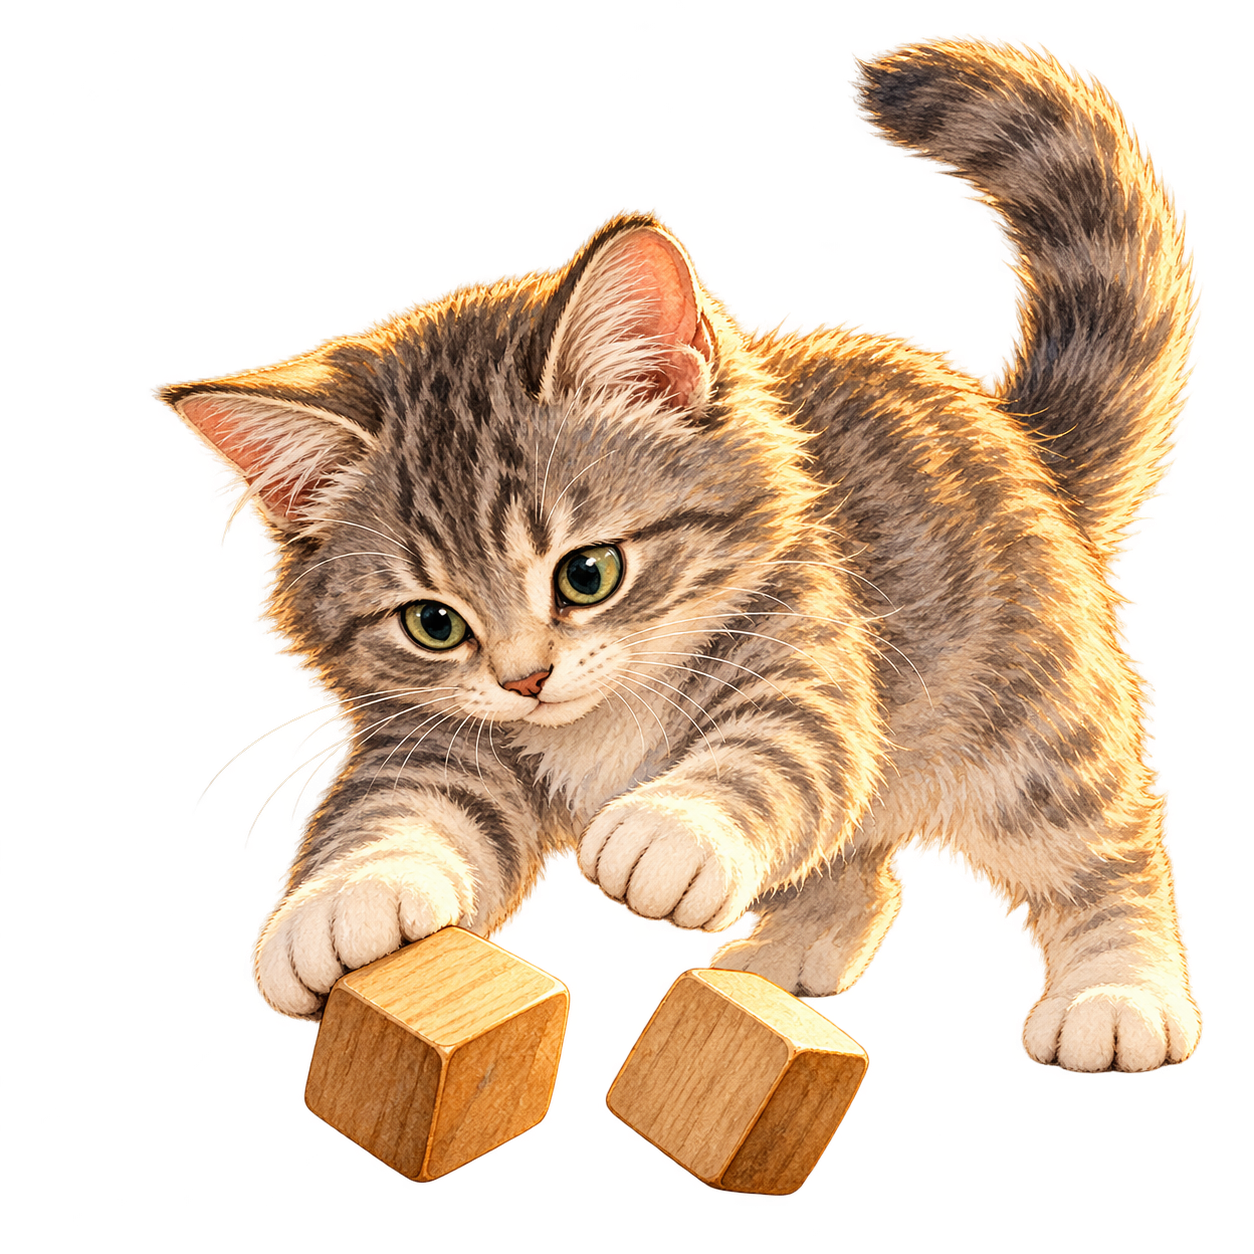
\includegraphics[width=54mm,height=58mm,keepaspectratio]{images/unique/art-17.png}
\end{wrapfigure}
\textit{Доказательство.} Для каждого результата первого шага имеется \(n_2\) продолжений. Получаются \(n_1\) непересекающихся групп по \(n_2\) исходов, всего \(n_1n_2\). Для большего числа шагов повторяем рассуждение, то есть применяем индукцию по числу шагов.\hfill\(\blacksquare\)

Например, к каждой из \(3\) рубашек можно надеть любые из \(2\) брюк:
получается \(3\cdot2=6\) комплектов.
Если число продолжений зависит от сделанного выбора, ветви сначала считают отдельно,
а затем складывают.
\par\WFclear\end{minipage}\end{lrbox}%
\ifdim\dimexpr\ht\CatFlowBox+\dp\CatFlowBox\relax<64mm\dp\CatFlowBox=\dimexpr64mm-\ht\CatFlowBox\relax\fi%
\noindent\usebox{\CatFlowBox}\par\addvspace{5pt}
\section{Факториал и перестановки}

\begin{definition}
\term{Факториал} (factorial) натурального числа \(n\) --- произведение всех натуральных чисел от \(1\) до \(n\):
\[
n!=1\cdot2\cdots n.
\]
Дополнительно полагают \(0!=1\). Поэтому для \(n\in\mathbb N_0\)
\[
(n+1)!=(n+1)n!.
\]
\end{definition}

Значение \(0!=1\) соответствует одному способу расположить ноль элементов:
получить пустую последовательность. Например, \(4!=24\).

\begin{definition}
\term{Перестановка без повторений} (permutation without repetition) ---
расположение всех \(n\) различных элементов в определённом порядке.
\end{definition}

На первое место есть \(n\) вариантов, на второе --- \(n-1\), и так далее.
По правилу произведения число перестановок равно
\[
P_n=n!.
\]

\begin{definition}
\term{Перестановка с повторениями} (multiset permutation) ---
расположение \(n\) элементов, среди которых есть одинаковые:
\(n_1\) элементов первого вида, \(n_2\) второго и так далее,
где \(n_1+\cdots+n_r=n\).
\end{definition}

Число таких перестановок равно
\[
P(n_1,\ldots,n_r)=\frac{n!}{n_1!\cdots n_r!}.
\]
Действительно, если временно различить все одинаковые элементы,
каждое конечное расположение будет учтено \(n_1!\cdots n_r!\) раз.
Например, из букв слова «МАМА» получается \(\frac{4!}{2!2!}=6\) разных последовательностей.

\section{Размещения: порядок важен}

\begin{definition}
\term{Размещение без повторений} (ordered selection without repetition) ---
упорядоченный выбор \(k\) различных элементов из \(n\) различных элементов.
\end{definition}

Для \(0\le k\le n\) число размещений равно
\[
A_n^k=\frac{n!}{(n-k)!}.
\]
При \(k\ge1\) это произведение \(k\) множителей:
\(n(n-1)\cdots(n-k+1)\); при \(k=0\) имеется один пустой выбор.
Например, капитана и заместителя из \(5\) человек выбирают \(A_5^2=5\cdot4=20\) способами.

\begin{definition}
\term{Размещение с повторениями} (ordered selection with repetition) ---
последовательность длины \(k\), каждый элемент которой выбирают из \(n\) видов;
один и тот же вид можно выбирать несколько раз.
\end{definition}

При \(n\ge1\), \(k\in\mathbb N_0\) число таких последовательностей равно
\[
\overline A_n^k=n^k.
\]
Например, двухсимвольных кодов из букв \(A,B,C\) ровно \(3^2=9\):
\(AA,AB,AC,BA,BB,BC,CA,CB,CC\).

\section{Сочетания: порядок не важен}

\begin{definition}
\term{Сочетание без повторений} (combination without repetition) ---
выбор \(k\) элементов из \(n\) различных элементов, при котором порядок не учитывается
и каждый элемент выбирают не более одного раза.
\end{definition}

Каждый такой выбор порождает \(k!\) размещений, поэтому
\[
C_n^k=\binom nk=\frac{n!}{k!(n-k)!},\qquad 0\le k\le n.
\]
Например, пару участников из \(5\) человек выбирают \(\binom52=10\) способами.
Здесь обмен участников местами не создаёт новую пару.

\begin{definition}
\term{Сочетание с повторениями} (combination with repetition) ---
выбор \(k\) элементов из \(n\) видов, при котором порядок не учитывается,
а элементы каждого вида можно брать в любом количестве.
\end{definition}

При \(n\ge1\), \(k\in\mathbb N_0\) число таких выборов равно
\[
\overline C_n^k=\binom{n+k-1}{k}=\binom{n+k-1}{n-1}.
\]
Выбор задаётся количествами \(x_1,\ldots,x_n\) элементов каждого вида:
\(x_i\in\mathbb N_0\), \(x_1+\cdots+x_n=k\).
Чтобы увидеть формулу, расположим в строку \(k\) одинаковых звёздочек и \(n-1\) перегородок.
Количество звёздочек до первой перегородки задаёт \(x_1\), между первой и второй --- \(x_2\), и так далее.
Перегородки могут стоять рядом и по краям: это соответствует нулевым количествам.
Нужно выбрать позиции \(n-1\) перегородок среди \(n+k-1\) позиций.
Например, для \(3\) видов и \(4\) элементов получается \(\binom62=15\) выборов.

\section{Биномиальные коэффициенты}

\begin{definition}
\term{Биномиальный коэффициент} (binomial coefficient) \(\binom nk\)
--- число сочетаний без повторений из \(n\) элементов по \(k\).
\end{definition}

Непосредственно из смысла выбора следуют равенства
\[
\binom n0=\binom nn=1,\qquad
\binom nk=\binom n{n-k}.
\]
Последнее равенство выражает соответствие между выбранными \(k\) элементами
и \(n-k\) оставшимися.

\begin{theorem}[Тождество Паскаля (Pascal's identity)]\label{thm:legacy-c10-3}
Для целых \(n\ge1\), \(1\le k\le n\)
\[
\binom{n+1}k=\binom n{k-1}+\binom nk.
\]
\end{theorem}

\begin{proof}
Выделим один элемент из \(n+1\) различных элементов.
Если он входит в выбранную группу из \(k\) элементов,
остальных участников выбирают \(\binom n{k-1}\) способами.
Если не входит, всю группу выбирают \(\binom nk\) способами.
Эти случаи не пересекаются и охватывают все группы; применяем правило суммы.
\end{proof}

\section{Бином Ньютона}

\begin{theorem}[Бином Ньютона (binomial theorem)]\label{thm:legacy-c10-4}
Для любых рациональных чисел \(a,b\) и любого натурального \(n\)
\[
(a+b)^n=a^n+\sum_{k=1}^{n-1}\binom nk a^{n-k}b^k+b^n.
\]
Знак \(\sum\) означает сложение слагаемых при всех указанных значениях индекса \(k\).
При \(n=1\) внутренняя сумма пуста и равна нулю, так что формула даёт \(a+b=a+b\).
\end{theorem}

\par\addvspace{5pt}\begin{lrbox}{\CatFlowBox}\begin{minipage}[t]{\linewidth}
\setlength{\parskip}{5pt}\setlength{\columnsep}{4.5mm}\setlength{\intextsep}{0pt}
\begin{wrapfigure}[12]{r}{54mm}

\includegraphics[width=54mm,height=58mm,keepaspectratio]{images/unique/art-18.png}
\end{wrapfigure}
\textit{Доказательство.} Раскроем произведение \(n\) одинаковых скобок \((a+b)\).
В каждом слагаемом из каждой скобки выбран либо \(a\), либо \(b\).
Если при \(1\le k\le n-1\) число \(b\) выбрано ровно из \(k\) скобок,
а \(a\) --- из остальных, получается \(a^{n-k}b^k\).
Нужные \(k\) скобок можно выбрать \(\binom nk\) способами.
Выбор только \(a\) даёт \(a^n\), выбор только \(b\) --- \(b^n\).
Собирая одинаковые слагаемые, получаем формулу.\hfill\(\blacksquare\)
\par\WFclear\end{minipage}\end{lrbox}%
\ifdim\dimexpr\ht\CatFlowBox+\dp\CatFlowBox\relax<64mm\dp\CatFlowBox=\dimexpr64mm-\ht\CatFlowBox\relax\fi%
\noindent\usebox{\CatFlowBox}\par\addvspace{5pt}


Например,
\[
(a+b)^3=a^3+3a^2b+3ab^2+b^3.
\]
Запись с отдельно выписанными крайними слагаемыми позволяет применять формулу
и при \(a=0\) или \(b=0\), не вводя выражение \(0^0\).

\section{Примеры: порядок выбора и коэффициент бинома}
\begin{example}Из восьми человек выбирают двух дежурных с одинаковыми обязанностями: \(C_8^2=28\). Если выбирают старосту и заместителя, роли различны: \(8\cdot7=56\). Каждой неупорядоченной паре соответствуют два распределения ролей. Возвращение одного человека в выбор здесь не разрешено.\end{example}
\begin{example}Коэффициент при \(x^2\) в \((1+2x)^4\) равен \(C_4^2\cdot2^2=24\): выбираем ровно два множителя, из которых берём \(2x\), из остальных берём единицу. Член бинома Ньютона имеет вид \(C_4^k(2x)^k\), поэтому степень аргумента определяет индекс \(k\).\end{example}
\Needspace{7\baselineskip}\section*{Задачи}
\begingroup\setlength{\parskip}{2pt}
\noindent\begin{minipage}[t]{\linewidth}\textbf{14.1.} На полке стоят \(5\) разных романов и \(3\) разных учебника. Сколько есть способов выбрать одну книгу?\par\end{minipage}\par
\noindent\begin{minipage}[t]{\linewidth}\textbf{14.2.} Есть \(4\) рубашки, \(3\) пары брюк и \(2\) пары обуви. Любые вещи можно сочетать. Сколько комплектов из одной рубашки, одной пары брюк и одной пары обуви можно составить?\par\end{minipage}\par
\noindent\begin{minipage}[t]{\linewidth}\textbf{14.3.} Для каждого выбора укажи, важен ли порядок и разрешены ли повторения: а) распределить три призовых места между \(10\) участниками без ничьих; б) выбрать команду из \(3\) человек среди \(10\); в) составить код длины \(3\) из цифр \(0,\ldots,9\), допуская одинаковые цифры; г) выбрать \(3\) элемента из \(4\) видов, допуская один вид несколько раз и не учитывая порядок.\par\end{minipage}\par
\noindent\begin{minipage}[t]{\linewidth}\textbf{14.4.} Вычисли \(5!\), \(0!\) и \(\dfrac{7!}{5!}\).\par\end{minipage}\par
\noindent\begin{minipage}[t]{\linewidth}\textbf{14.5.} Сколькими способами можно расположить в ряд \(6\) различных книг, используя каждую ровно один раз?\par\end{minipage}\par
\noindent\begin{minipage}[t]{\linewidth}\textbf{14.6.} Сколько разных последовательностей можно получить, переставляя все буквы слова «ТОПОТ»? Осмысленность полученных слов не требуется.\par\end{minipage}\par
\noindent\begin{minipage}[t]{\linewidth}\textbf{14.7.} В забеге участвуют \(8\) человек. Сколько существует вариантов распределения первого, второго и третьего мест, если ничьи невозможны?\par\end{minipage}\par
\noindent\begin{minipage}[t]{\linewidth}\textbf{14.8.} Из \(8\) различных элементов выбирают \(3\), не учитывая порядок. Сколько существует выборов?\par\end{minipage}\par
\noindent\begin{minipage}[t]{\linewidth}\textbf{14.9.} Электронный замок принимает код из \(4\) цифр от \(0\) до \(9\). Повторения разрешены, первая цифра может быть нулём. Сколько разных кодов возможно?\par\end{minipage}\par
\noindent\begin{minipage}[t]{\linewidth}\textbf{14.10.} Сколько существует четырёхзначных натуральных чисел с попарно различными цифрами?\par\end{minipage}\par
\noindent\begin{minipage}[t]{\linewidth}\textbf{14.11.} Из \(4\) видов элементов выбирают \(3\) элемента. Каждый вид можно использовать сколько угодно раз, порядок не учитывается. Сколько существует выборов?\par\end{minipage}\par
\noindent\begin{minipage}[t]{\linewidth}\textbf{14.12.} Сколькими способами можно разложить \(7\) одинаковых шаров по \(3\) различным ящикам? Пустые ящики допускаются.\par\end{minipage}\par
\noindent\begin{minipage}[t]{\linewidth}\textbf{14.13.} Из множества, состоящего из \(n\ge2\) элементов, можно выбрать ровно \(45\) различных неупорядоченных пар. Найди \(n\).\par\end{minipage}\par
\par\addvspace{5pt}\begin{lrbox}{\CatFlowBox}\begin{minipage}[t]{\linewidth}
\setlength{\parskip}{5pt}\setlength{\columnsep}{4.5mm}\setlength{\intextsep}{0pt}
\begin{wrapfigure}[12]{l}{54mm}

\includegraphics[width=54mm,height=58mm,keepaspectratio]{images/unique/art-29.png}
\end{wrapfigure}
\textbf{14.14.} Пользуясь тождеством Паскаля и значениями \(\binom72=21\), \(\binom73=35\), вычисли \(\binom83\).\par

\textbf{14.15.} Раскрой скобки в \((x+2)^4\) с помощью бинома Ньютона.\par

\textbf{14.16.} Найди коэффициент при \(x^3\) после раскрытия скобок в \((2+x)^7\).\par

\textbf{14.17.} Докажи, что для любого \(n\in\mathbb N_0\) выполняется \(\sum_{k=0}^{n}\binom nk=2^n\).\par

\textbf{14.18.}\starmark{} Из \(4\) девушек и \(6\) юношей выбирают группу из \(5\) человек. Сколько существует групп, в которых не меньше двух девушек?\par

\textbf{14.19.}\starmark{} Сколько кодов длины \(5\) из цифр \(0,\ldots,9\) содержат хотя бы один ноль и хотя бы одну единицу? Начальный ноль разрешён, повторения разрешены.\par

\textbf{14.20.}\starmark{} Докажи подсчётом одного и того же множества двумя способами тождество Вандермонда: \(\sum_{k=0}^{r}\binom mk\binom n{r-k}=\binom{m+n}{r}\), где \(m,n\in\mathbb N_0\), \(0\le r\le m+n\). В этой задаче \(\binom uv=0\), если целое \(v<0\) или \(v>u\). Рассматривай целое \(r\in\mathbb N_0\).\par
\par\WFclear\end{minipage}\end{lrbox}%
\ifdim\dimexpr\ht\CatFlowBox+\dp\CatFlowBox\relax<64mm\dp\CatFlowBox=\dimexpr64mm-\ht\CatFlowBox\relax\fi%
\noindent\usebox{\CatFlowBox}\par\addvspace{5pt}

\endgroup
